\documentclass[a4paper,oneside]{article}

\usepackage[utf8]{inputenc}
\usepackage[T2A]{fontenc}
\usepackage[english,russian]{babel}

\usepackage{amsmath}
\usepackage{mathtools}
\usepackage{amsfonts}
\usepackage{enumitem}
\usepackage{amsthm}
\usepackage{minted}
\setminted{fontsize=\small, breaklines=true, style=emacs, linenos}
\usepackage{graphicx}
\graphicspath{ {./images/} }
\usepackage{float}

\newtheorem{theorem}{Теорема}[subsection]
\newtheorem*{theorem*}{Теорема}

% --- Определение --- %
\theoremstyle{definition}
\newtheorem{definition}{Определение}[subsection]
\newtheorem*{definition*}{Определение}
% ------------------- %

\title{{Теория кодирования и сжатия информации}\\{Лабораторная работа №7}}
\author{Гущин Андрей, 431 группа, 1 подгруппа}
\date{\the\year{} г.}

\begin{document}

\maketitle

\section{Задача}

Разработать программу осуществляющую архивацию и разархивацию текстового файла
используя алгоритм Лемпеля-Зива (LZ77). Программы архивации и разархивации
должны быть представлены отдельно и работать независимо друг от друга.
Определить для данного шифра характеристики 1 (коэффициент сжатия) и 2 (скорость
сжатия). К работе необходимо прикрепить отчет и программный проект.


\section{Алгоритм}

Алгоритм LZ77 заключается в создании нового кода для всех встречающихся
последовательностей символов. Алгоритм использует идею <<скользящего окна>>
для создания кодов.

Алгоритм состоит из следующих шагов:
\begin{enumerate}
  \item
    Прочитать первый символ. Так как он ни разу не встречался, закодировать его
    как (0, 0, ?), где (offset, l, char), offset --- сдвиг относительно текущей
    позиции, l --- длина последовательности, char --- символ, стоящий после
    последовательности.
  \item
    Далее необходимо найти наибольшую подстроку ps, начинающуюся в окне и
    при этом равную подстроке, начинающейся в текущей позиции.
  \item
    Если строка не найдена, то просто добавить отдельный символ аналогично
    самому первому. Иначе закодировать с помощью сдвига и чтения подстроки
    длины $l$.
  \item
    Если при чтении кода встретилась записи длины 0, то необходимо просто
    добавить указанный символ.
  \item
    Иначе необходимо скопировать $l$ символов, начиная с $current - offset$, а
    после них добавить один символ $char$.
\end{enumerate}


\section{Тестирование}

Для проверки программы были использованы тестовые тексты 1 (рис.
\ref{fig:test_1}) и 6 (рис. \ref{fig:test_6}). Можно заметить,
что после распаковки архива полученный файл совпадает с исходным (проверка
с помощью утилиты diff). Также можно заметить, что для файлов малого размера
архив увеличивает их размер за счёт метаданных.

\begin{figure}[H]
  \centering
  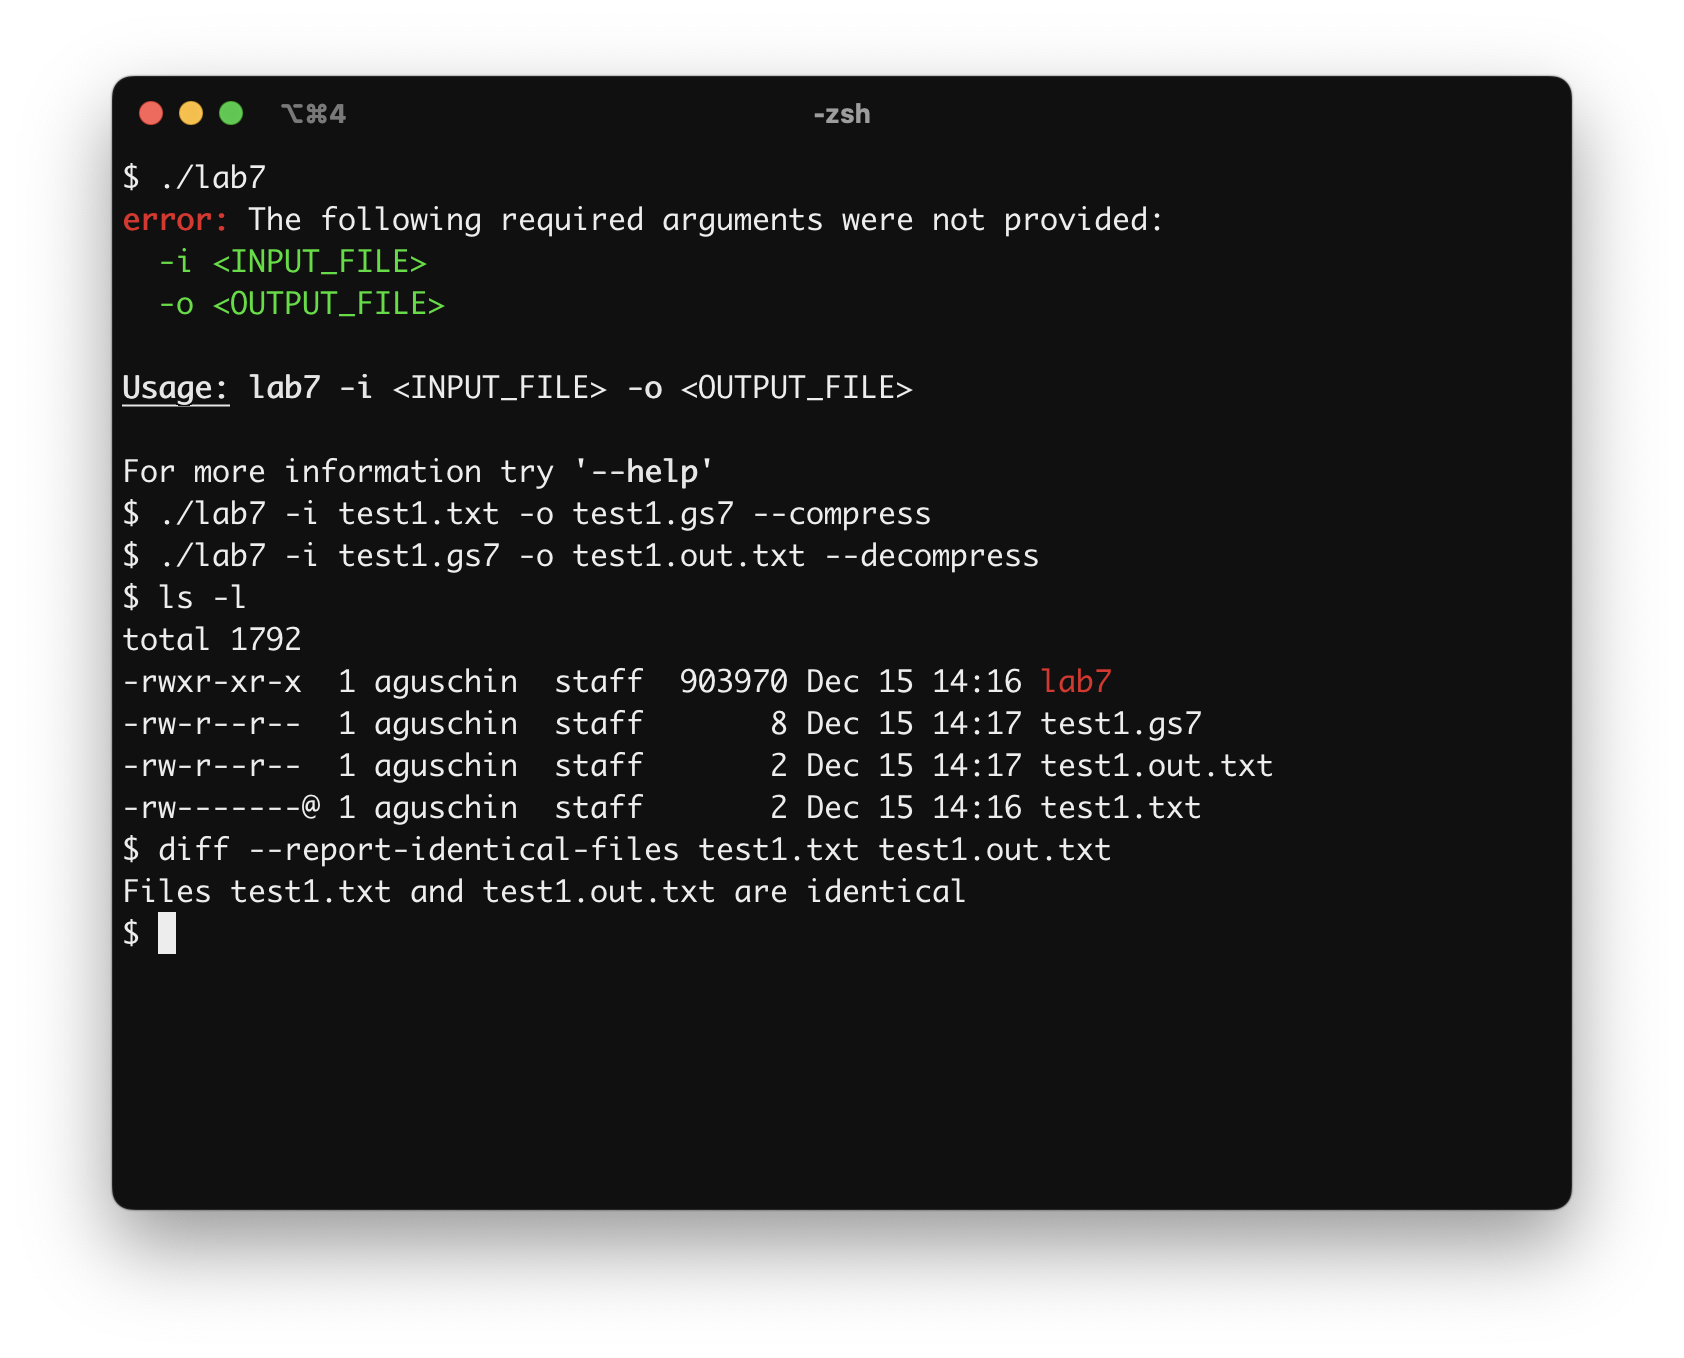
\includegraphics[width=0.9\textwidth]{test1.png}
  \caption{Сжатие текста Тест\_1.txt}
  \label{fig:test_1}
\end{figure}

\begin{figure}[H]
  \centering
  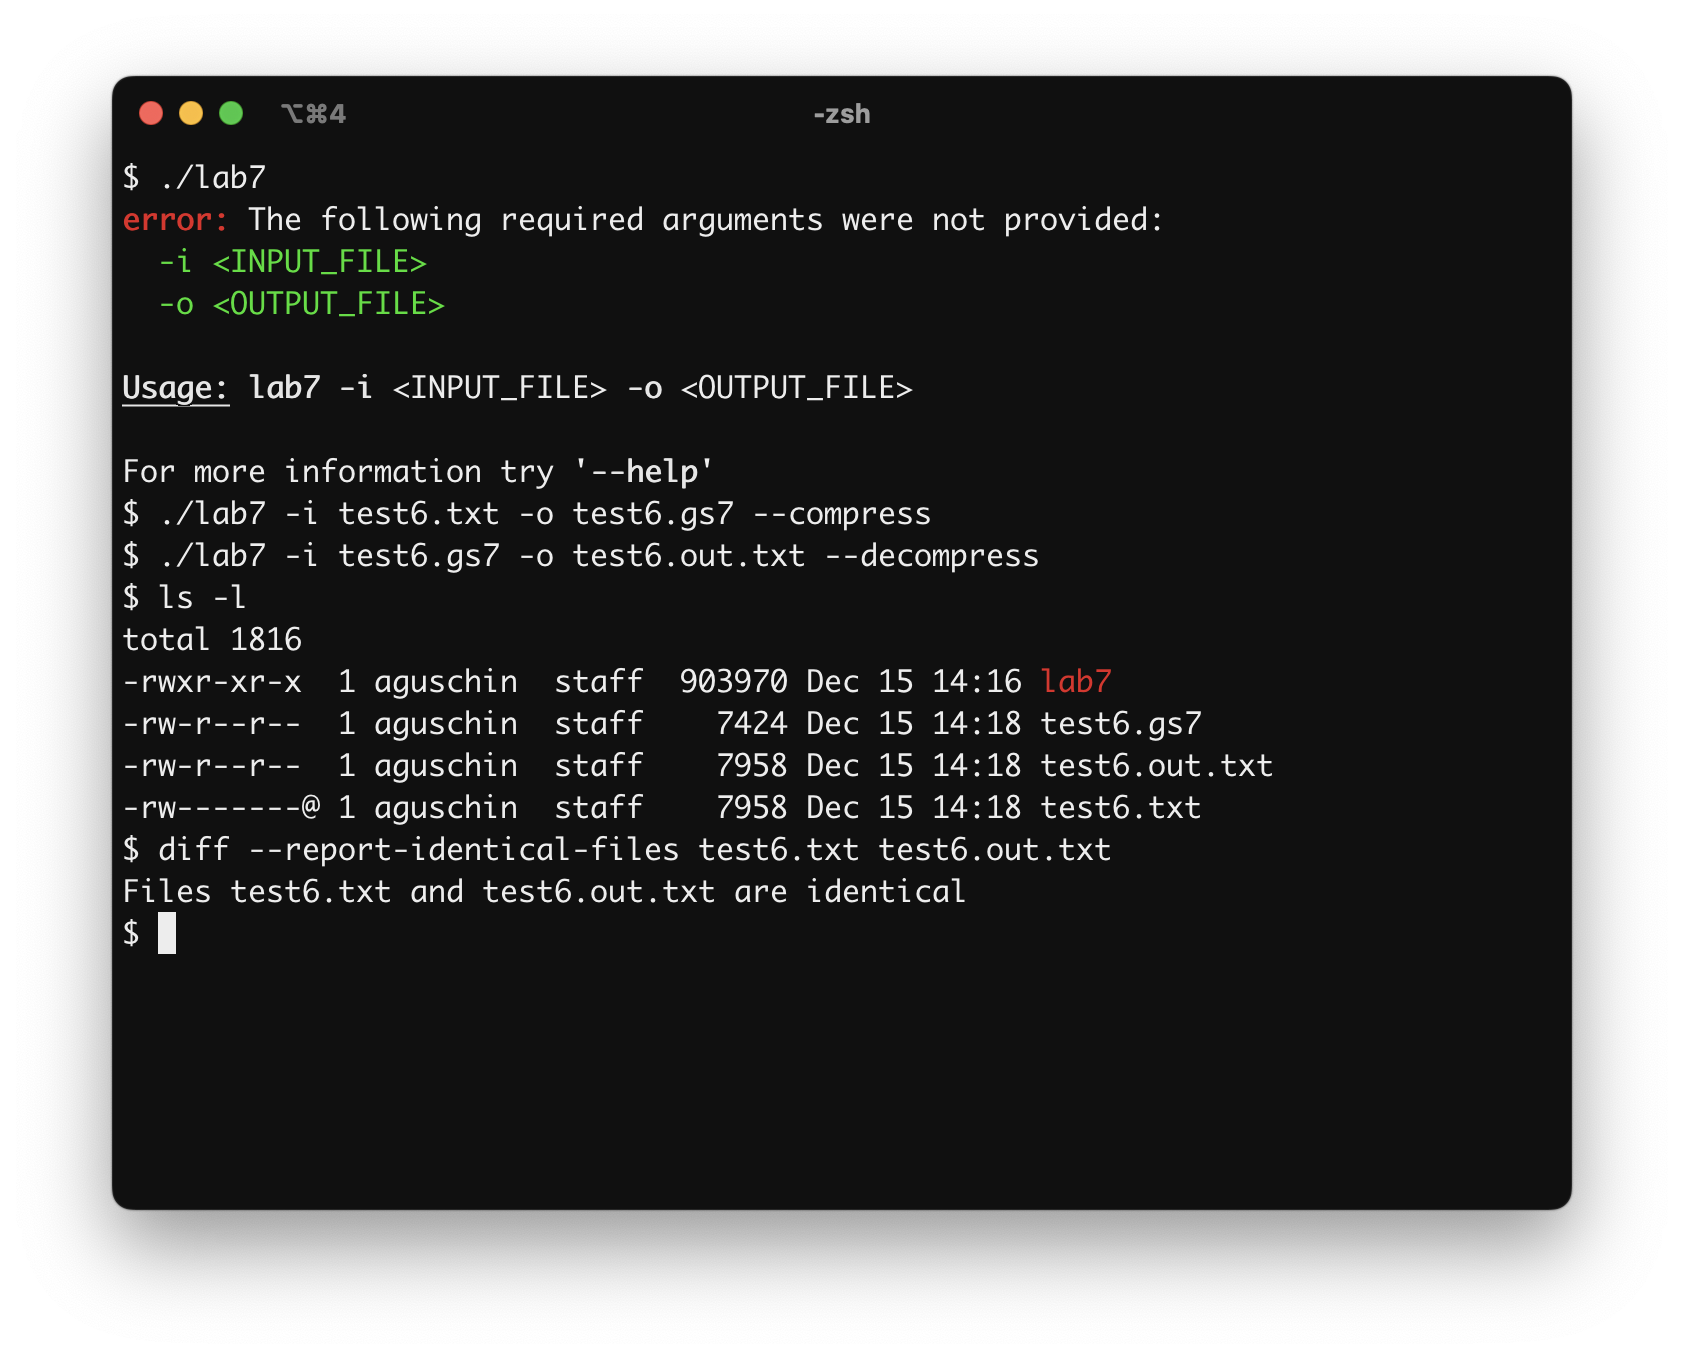
\includegraphics[width=0.9\textwidth]{test6.png}
  \caption{Сжатие текста Тест\_6.txt}
  \label{fig:test_6}
\end{figure}


\section{Вычисленные характеристики}

\subsection{Характеристика 1 (Коэффициент сжатия)}

Результаты применения программы к каждому из тестовых текстовых файлов занесены
в таблицу \ref{tbl:results}.

\begin{table}[H]
  \small
  \centering
  \begin{tabular}{|c|c|c|c|}
    \hline
    Название     & Исходный размер, байт & Сжатый размер, байт & Коэффициент \\ \hline \hline
    Тест\_1.txt  & 2           &      8      & 0.25    \\ \hline
    Тест\_2.txt  & 33          &    132      & 0.25    \\ \hline
    Тест\_3.txt  & 2739        &    176      & 15.5625 \\ \hline
    Тест\_4.txt  & 330         &     16      & 20.625  \\ \hline
    Тест\_5.txt  & 59          &    236      & 0.25    \\ \hline
    Тест\_6.txt  & 7958        &   7424      & 1.68459 \\ \hline
    Тест\_7.txt  & 138245      & 104980      & 1.31687 \\ \hline
    Тест\_8.txt  & 574426      & 415612      & 1.38212 \\ \hline
    Тест\_9.txt  & 2752        &     48      & 57.3333 \\ \hline
    Тест\_10.txt & 2814        &     56      & 50.25   \\ \hline
  \end{tabular}
  \caption{результаты тестирования}
  \label{tbl:results}
\end{table}

\subsection{Характеристика 2 (Скорость сжатия)}

Для тестирования скорости сжатия использовался произвольный двоичный
файл размера 3120002 байт ($\approx$3 мегабайта). В результате пяти
последовательных запусков, среднее время запаковки файла составило 17.23
секунды, среднее время распаковки составило 0.02 секунд.

Таким образом, средняя скорость сжатия составила 0.17269 Мбайт в секунду, а
средняя скорость разжатия составила 148.77329 Мбайт в секунду.

\section{Реализация}

Программа реализована на языке программирования Rust с использованием библиотеки
clap для чтения параметров командной строки. Сборка производится с помощью
программы cargo, поставляющейся вместе с языком.

\subsection{Содержимое файла lz77.rs}
\inputminted{rust}{../../lab7/src/lz77.rs}

\subsection{Содержимое файла main.rs}
\inputminted{rust}{../../lab7/src/main.rs}

\subsection{Содержимое файла Cargo.toml}
\inputminted{toml}{../../lab7/Cargo.toml}

\end{document}
